\section{Introducción}
La flauta es un instrumento de viento-madera en forma de tubo. Tiene
3 partes: base, cuerpo y cabeza. La flauta tiene ocho agujeros: siete
delante y uno detrás. Estos agujeros se numeran, siendo el 0 el agujero
de atrás y el 7 el de más abajo. A cada agujero le corresponde un
dedo. Se tapan y se destapan con la yema de los dedos, pero sin apretar.
Los agujeros 0, 1, 2 y 3 se tapan con la mano izquierda: el pulgar
tapa el 0, el índice el 1, medio el 2, y anular el 3. El resto de
agujeros se tapan con la mano derecha: el índice el 4, medio el 5,
anular el 6 y meñique el 7. El dedo pulgar derecho se coloca entre
los agujeros 4 y 5 por detrás de la flauta. Aunque no tapa ningún
agujero, sirve para soportar el peso de la flauta. Se puede mostrar
en la siguiente imagen.
\begin{figure}[H]
	\begin{center}
		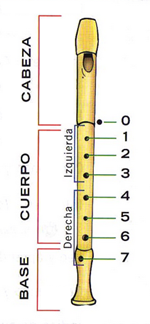
\includegraphics[scale=.8]{img/flauta.png}
		\caption{Composición de una flauta dulce}
		\label{fig:tabla0}
	\end{center}
\end{figure}
Para poder tocar las notas musicales en la flauta se deben colocar
los dedos en los distintos agujeros de la manera en que se muestran
en la siguiente imagen.
\begin{figure}[H]
	\begin{center}
		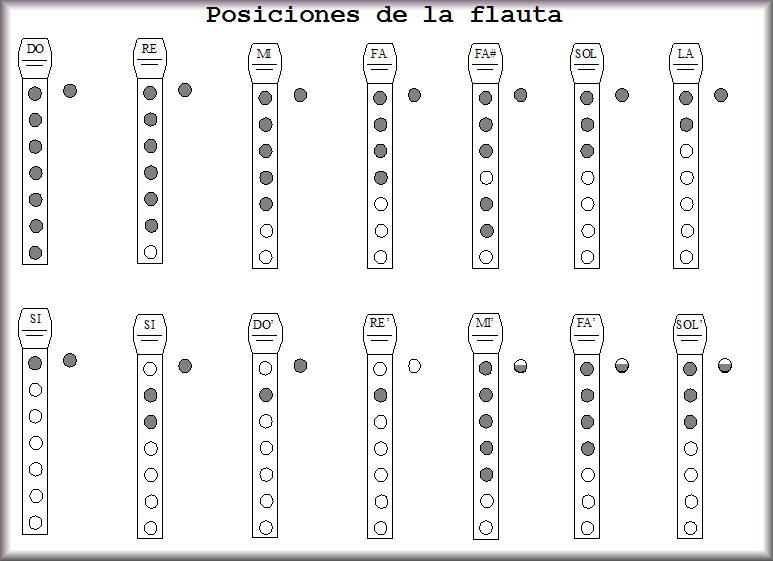
\includegraphics[scale=.35]{img/posiciones_de_la_flauta.png}
		\caption{Posiciones de la flauta para tocar diversas notas}
		\label{fig:tablas}
	\end{center}
\end{figure}

Los agujeros grises mostrados en la figura son los agujeros que deben
ser tapados por los dedos y los agujeros blancos son los que no se
deben tapar para poder hacer sonar esa nota musical. Las notas que
tienen un apostrofe son notas más agudas, es decir, están en la segunda
octava que puede tocar la flauta. Las notas musicales son 7: Do, Re,
Mi, Fa, Sol, La y Si. Entre ellas hay notas que se consiguen ya sea
con sostenidos o bemoles. Si quieren notas más graves o agudas que
las 7 anteriores o sus intermedias, utilizo el nombre de las mismas
notas para los tonos más altos o más graves. Por supuesto que no será
la misma nota en la práctica, al escuchar el tono; pero se utilizarán
los mismos nombres diciendo que la nota está en otra octava. De este
modo tenemos notas de Do a Si, en la siguiente octava nuevamente de
Do a Si, luego la octava siguiente de Do a Si, y así sucesivamente
todo dentro del rango humanamente audible. En cuanto a las propiedades
del sonido, no es en vano que la octava de una nota tenga el mismo
nombre. La relación entre una nota y la siguiente del mismo nombre
en frecuencia de vibraciones, es decir, la siguiente nota del mismo
nombre, en la siguiente octava, vibra exactamente el doble de veces
que la anterior, es decir, si un \textquotedblleft La\textquotedblright{}
estándar de altura media es producto de 440 vibraciones por segundo,
el \textquotedblleft La\textquotedblright{} de la siguiente Octava
es físicamente algo vibrando 880 veces cada segundo, y el siguiente
\textquotedblleft La\textquotedblright{} producto de 1760 vibraciones
por segundo, esta vibraciones son los Hertz (Hz). En la siguiente
tabla se muestran las frecuencias que se pueden alcanzar según las
notas musicales, aunque la flauta únicamente alcanza las octavas 4
y 5, es decir, que la frecuencia mas chica que la flauta puede generar
es de 261.63 Hz y la nota mas aguda que puede generar es de 987.77
Hz. 
\begin{figure}[H]
	\begin{center}
		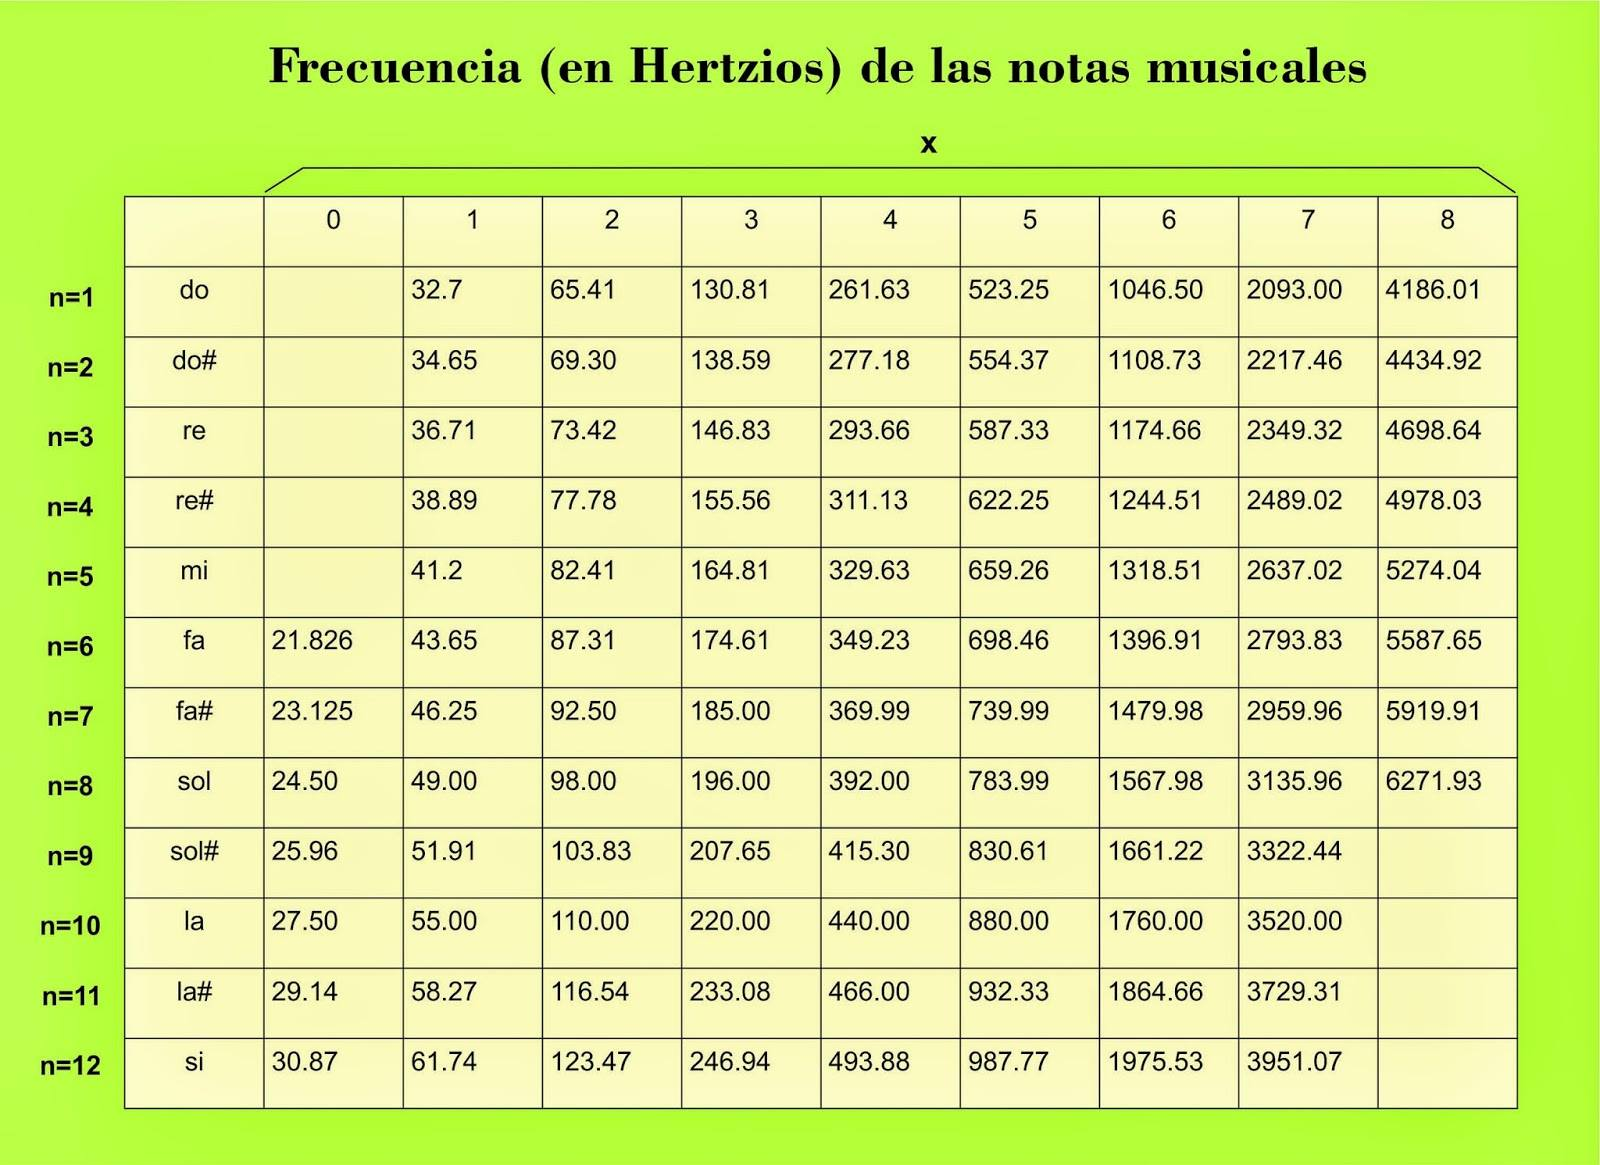
\includegraphics[scale=.24]{img/frecuencias.jpg}
		\caption{Frecuencias de las notas musicales}
		\label{fig:tabla1}
	\end{center}
\end{figure}

\paragraph{La transformada de Fourier}

Una transformada de Fourier es una operación matemática que transforma
una señal de dominio de tiempo a dominio de frecuencia y viceversa.
Estamos acostumbrados a señales con dominio de tiempo en la vida cotidiana.
En el dominio de tiempo, la señal se expresa con respecto al tiempo.
En el dominio de frecuencia, una señal es expresada con respecto a
la frecuencia. 

Una DFT (Transformada de Fourier Discreta - por sus siglas en inglés)
es el nombre dado a la transformada de Fourier cuando se aplica a
una señal digital (discreta) en vez de una análoga (continua). Una
FFT (Transformada Rápida de Fourier) es una versión más rápida de
la DFT que puede ser aplicada cuando el número de mustras de la señal
es una potencia de dos. Un cálculo de FFT toma aproximadamente N {*}
log2(N) operaciones, mientras que DFT toma aproximadamente N2 operaciones,
así es que la FFT es significativamente más rápida. 

La transformada discreta de Fourier (DFT) de una señal x{[}n{]} definidia
en el rango 0\textless{}=n\textless{}=N-1 se define como:\\

$x[k]=\sum x[n]*e^{-j\frac{2*\Pi}{N}*k*n}$; 0\textless{}=j\textless{}=N-1\\

\paragraph{Funcionamiento del Proyecto}
Este proyecto consiste en un programa que detecte las notas musicales
que son tocadas en una flauta dulce, el sonido que ésta produce será
grabado desde la computadora un tiempo N (el tiempo de la canción
que se desee tocar). al terminar la grabación, el programa se ejecuta para decir que nota fue tocada cada .064 segundos.\\
Esto es posible utilizando la FFT y evaluando la amplitud obtenida en frecuencia de los valores arrojados por la transformada.\\ La decisión de evaluar cada .064 segundos se debe a la frecuencia de muestreo escogida para realizar la grabación (4000 muestras/s, este valor fue obtenido por el teorema del muestreo) y la cantidad de muestras que se deseaban obtener. Al trabajar con la FFT era necesario que este total de muestras fuera una potencia de dos. Al dividir la grabación en fragmentos de .064 segundos se obtiene un total de 256 muestras, lo cual es suficiente para realizar el análisis con la resolución necesaria y empleando el menor número de muestras posible.